\documentclass{deliverablereport}
\usepackage{pdfpages}

\usepackage[style=alphabetic,backend=bibtex]{biblatex}
\addbibresource{../../lib/kbibs/kwarcpubs.bib}
\addbibresource{../../lib/kbibs/extpubs.bib}
\addbibresource{../../lib/kbibs/kwarccrossrefs.bib}
\addbibresource{../../lib/kbibs/extcrossrefs.bib}
\addbibresource{../../lib/deliverables.bib}
%\addbibresource{../../lib/publications.bib}
\addbibresource{rest.bib}
% temporary fix due to http://tex.stackexchange.com/questions/311426/bibliography-error-use-of-blxbblverbaddi-doesnt-match-its-definition-ve
\makeatletter\def\blx@maxline{77}\makeatother

\deliverable{component-architecture}{scscp-sage}
\deliverydate{02/27/2017}
\duedate{02/27/2017 (Month 18)}
\def\pn{OpenDreamKit}
\author{ }

\begin{document}
\maketitle
%  Work Package WP6 develops a novel, foundational, knowledge-based framework for
  interfacing existing open source mathematical software systems and knowledge bases into
  a mathematical VRE, where systems can delegate functionalities among each other
  seamlessly without losing semantics.

  The overall Math-in-the-Middle (MitM) Framework developed in WP6 over the last three
  years is described in D6.5; this Report complements it by describing the curated
  contents Math-in-the-Middle (MitM) Ontology which serves as a reference and pivotal
  point for translations between the various input languages of mathematical software
  systems and knowledge bases.

  In a nutshell, the MitM Ontology describes the mathematical objects, concepts, and their
  relations in a general, system-agnostic way in an OMDoc/MMT theory graph while the
  mathematical systems export API theories that describe the system interface language in
  terms of types, classes, constructors, and functions -- again in OMDoc/MMT. These two
  levels of descriptions are linked by OMDoc/MMT alignments that allow the translation of
  expressions between systems.

%%% Local Variables:
%%% mode: visual-line
%%% fill-column: 5000
%%% mode: latex 
%%% TeX-master: "report"
%%% End:

% TODO: replace GitHub issue description by the abstract?
\strut\githubissuedescription
\newpage\tableofcontents\newpage

\section{Introduction}\label{intro}

{\sf SCSCP} stands for the 
{\bf Symbolic Computation Software Composability Protocol}
-- the remote procedure call framework by which different
software components (primarily mathematical software systems) 
may offer computational services to a variety of possible
clients, such as, for example:
\begin{itemize}
\item A computer algebra system (CAS) running on the same computer system or remotely
\item Another instance of the same CAS (in a parallel computing context)
\item A simplistic SCSCP client (e.g. C/C++/Python/etc. program) with a minimal 
SCSCP support needed for a particular application
\item An internet application providing user interface to the computational services
\item A Web server which passes on the same services as Web services to other applications
\item Cloud middleware
\end{itemize}

SCSCP has been developed in the EU FP6 project 026133 
``SCIEnce'' TODO:title:URL) and initially has been
implemented in systems TODO:list. Later some other systems
joined the framework TODO:list, but not having implementations
for Python hindered further progress. 

Under the ODK project, we transferred SCSCP specification
to OpenMath society and licensed it under
W3C Software and document notice and license.

TODO:make a proper webpage for SCSCP under OpenMath VO, with
PDFs of the specification and links to existing implementations.


\section{Systems}\label{systems}

In OpenDreamKit, the task is to provide SCSCP implementations
for all involved components. SCSCP is a protocol in which 
both data and instructions are implemented in OpenMath, so
implementing SCSCP involves two tasks - implementing OpenMath
support to be able to parse and generate OpenMath code in order
to encode/decode mathematical objects, and on top of that 
then implementing necessary framework to establish connection,
send procedure calls and receive back results.

Instead of implementing it directly in SageMath, we have
decided that the maximal impact would be if we could provide
an independent Python library, which may be used then not
only in SageMath but also in a number of other Python applications
including scientific computing libraries such as e.g. NumPy,
SymPy etc. We will present this and other SCSCP implementations
below.


\subsection{GAP}

TODO: add URLs

GAP has two packages, SCSCP and OpenMath. The OpenMath package
provides encoding/decoding, supports both XML and binary OpenMath.
The SCSCP package implements SCSCP client and server, and on top of
that provides a framework for distributed parallel computations.

TODO: more details and either URLs of manuals or append them to the report?

During the reported period, we have prepared new versions of 
both packages. Packages were migrated under the GAP packages VO
on GitHub, their new versions are now picked up for the redistribution
with GAP and will appear in the next GAP release. Major changes
were upgrades and compatibility fixes for next GAP releases, 
and improvements to improve the security and robustness when
running public SCSCP servers. 

TODO: release GAP 4.8.7 by the end of February?

Several examples of using GAP SCSCP client and server are given
in the next section. They show how GAP SCSCP support feeds into
activities from other workpackages (Docker, databases).


\subsection{Python, SageMath and its components}

TODO: Ask Luca for descriptions of \url{https://github.com/OpenMath/py-scscp}
and \url{https://github.com/OpenMath/py-openmath}. 

Explain how the user can now use these packages to extend supported OpenMath CDs
or use private encodings and implement own remote procedures.

TODO: Appendix with READMEs from \url{https://github.com/OpenMath/py-scscp}
and \url{https://github.com/OpenMath/py-openmath}. The latter should have
some more detailed README.

Cover the whole ecosystem: SageMath and its components, other Python libraries.


\subsection{MMT/MathHub}

TODO: Ask Tom to provide a description



\section{Examples}\label{examples}

TODO: introduction to this section


\subsection{GAP SCSCP server in Docker container}

TODO: describe how one could run GAP SCSCP server
using GAP docker container 

https://hub.docker.com/r/gapsystem/gap-docker/ 

and possibly print that page or README from there in the appendix.


\subsection{Number of groups of order $n$}\label{gnu-reproducibility}

TODO: describe \url{https://github.com/alex-konovalov/gnu} which provides
an SCSCP server for the number of isomorphism types of groups. Provide
a GAP Jupyter notebook that talks to that server in the appendix.


\subsection{SageMath}

TODO: brief description, and reference to the appendix, extend examples


\subsection{Singular}

TODO: Sebastian?


\subsection{PARI/GP}

TODO: Via SageMath?


\subsection{Parallel SCSCP tutorial}

TODO: describe \url{https://github.com/alex-konovalov/scscp-demo},
include page in the appendix.

\section{Future work}

Dissemination: reach out to SymPy, NumPy, ...


\printbibliography

\appendix
\section{Example of SCSCP client in Python2 connecting to GAP server}
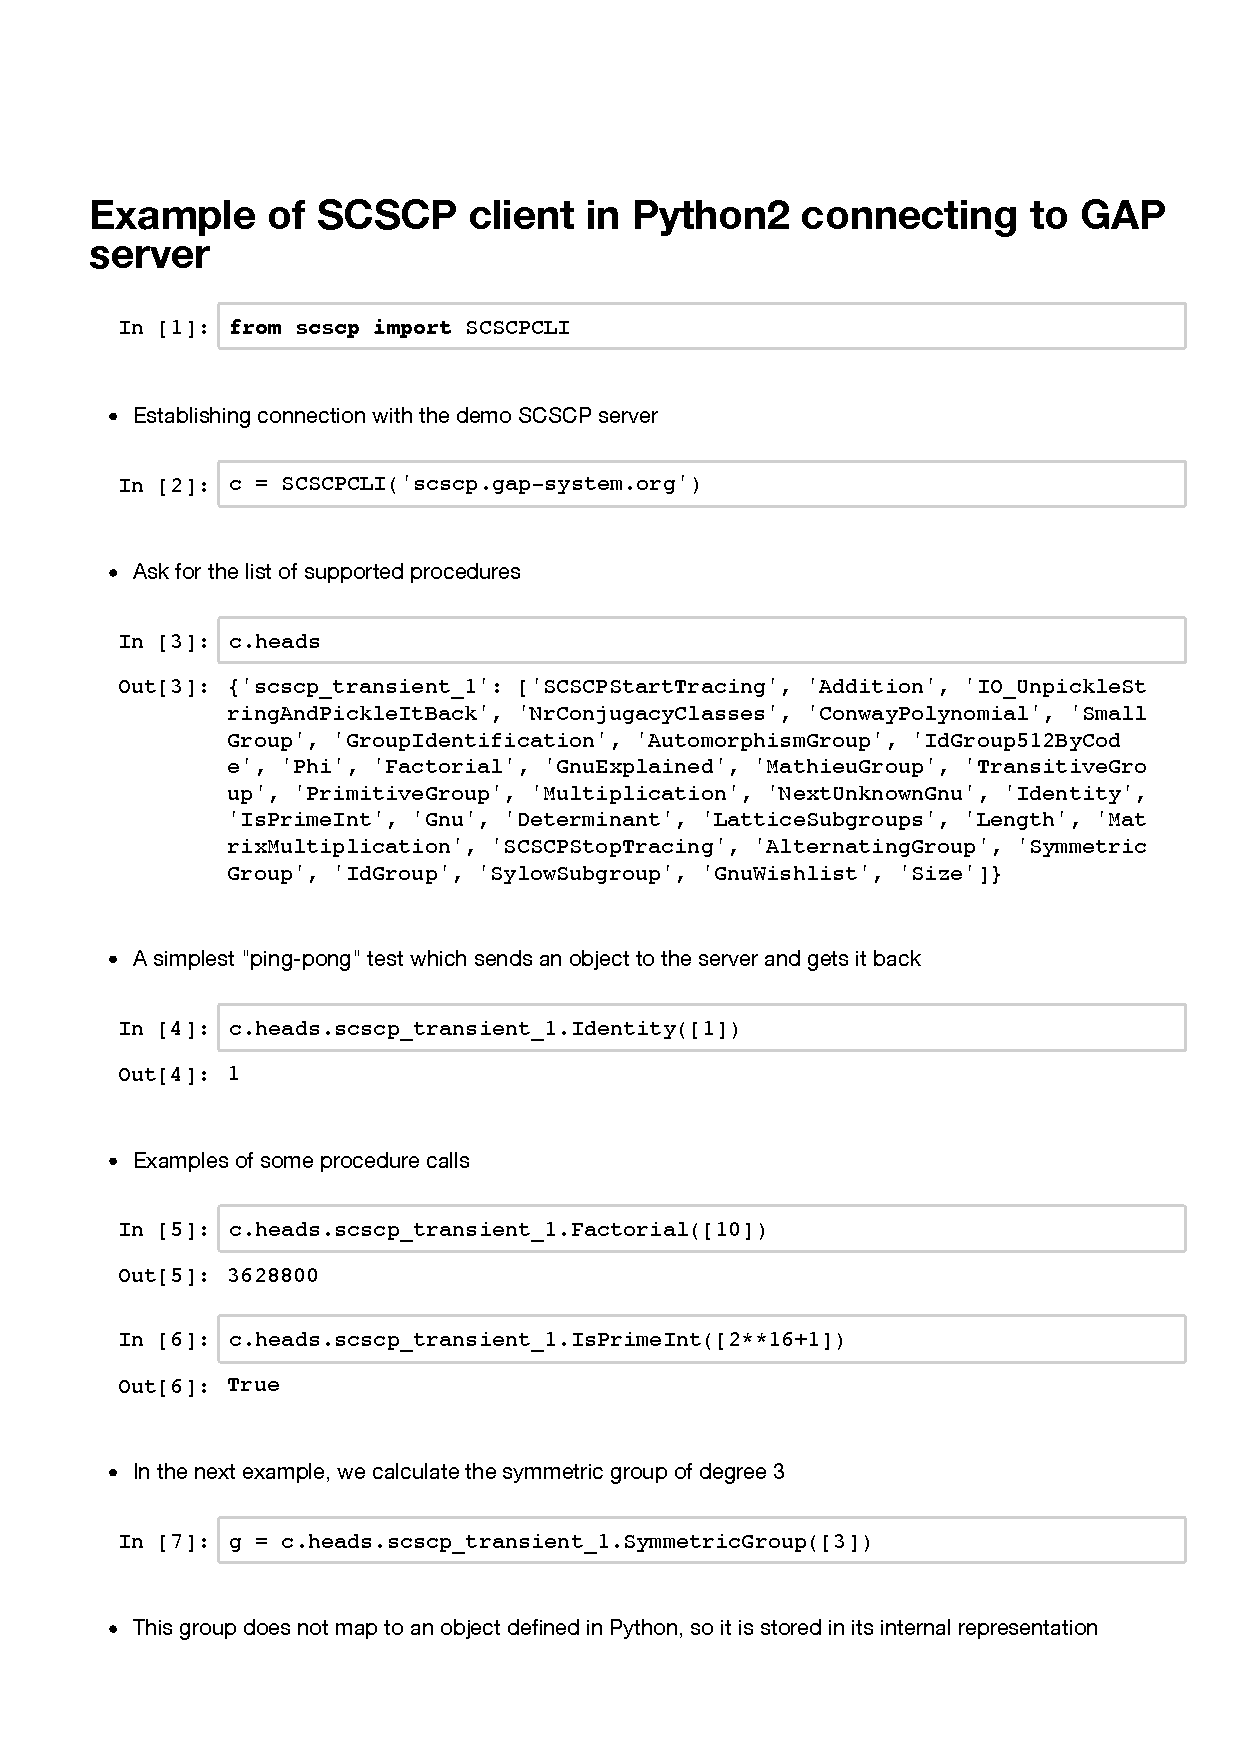
\includepdf[pages=-,scale=0.9,pagecommand={}]{examples/Python2-to-GAP.pdf}
\section{Example of SCSCP client in Python3 connecting to GAP server}
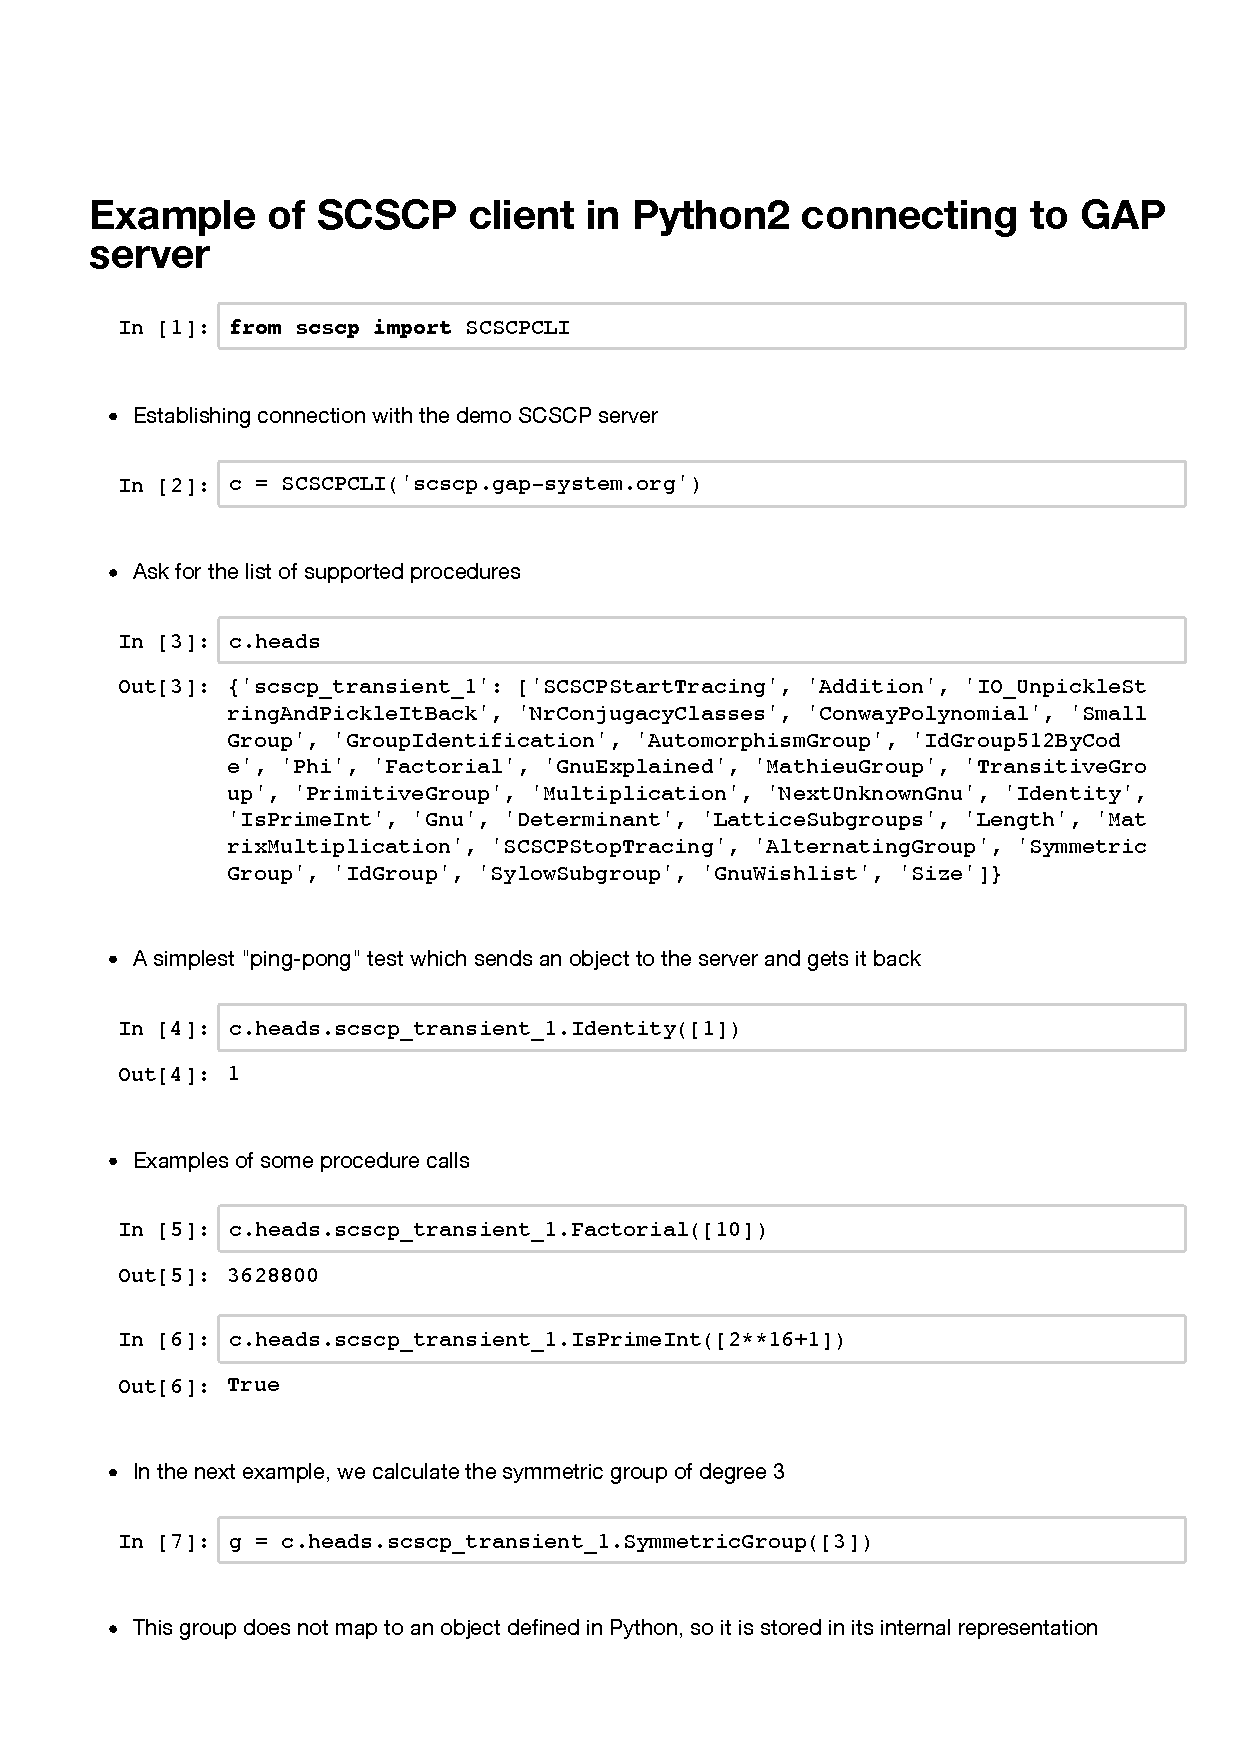
\includepdf[pages=-,scale=0.9,pagecommand={}]{examples/Python2-to-GAP.pdf}
\section{Example of SCSCP client in SageMath connecting to GAP server}
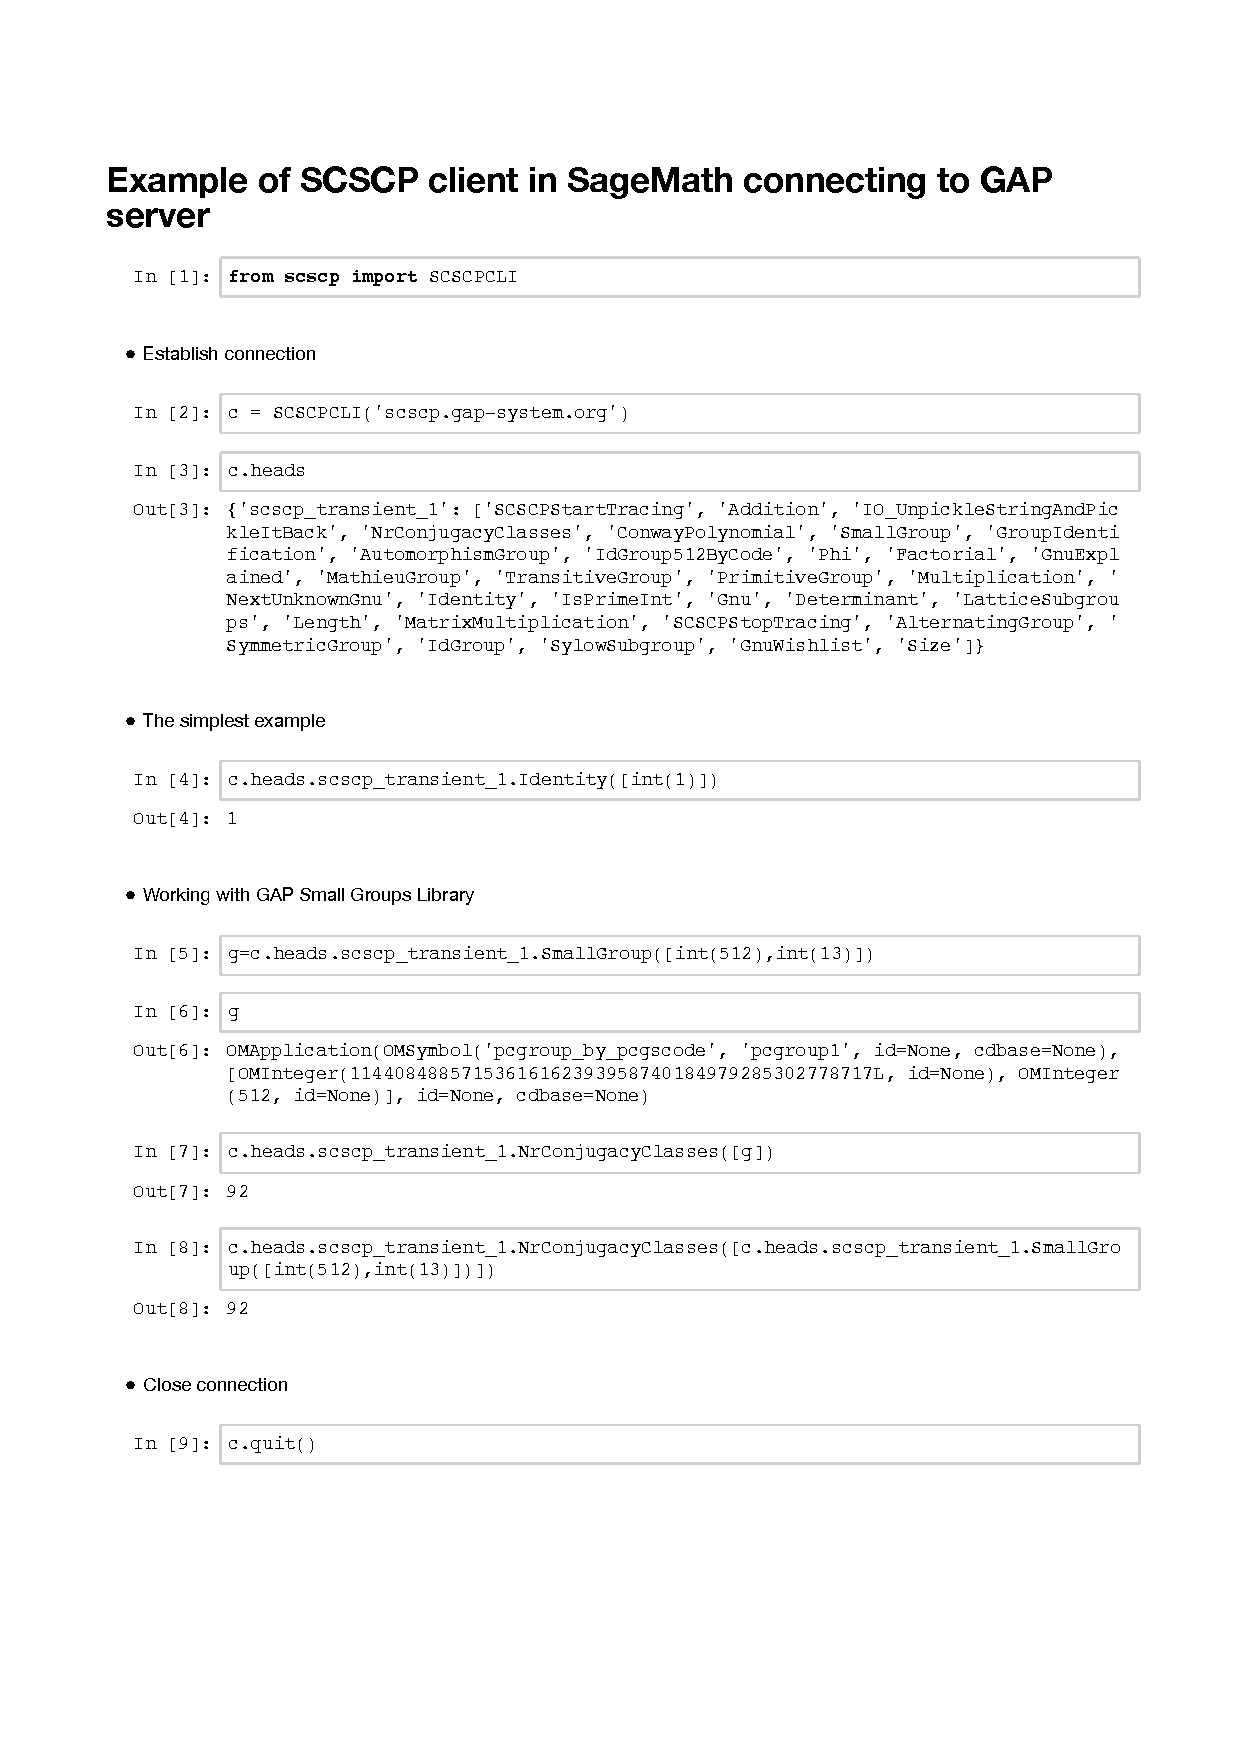
\includepdf[pages=-,scale=0.9,pagecommand={}]{examples/SageMath-to-GAP.pdf}
\section{Documentation on GAP Docker container}
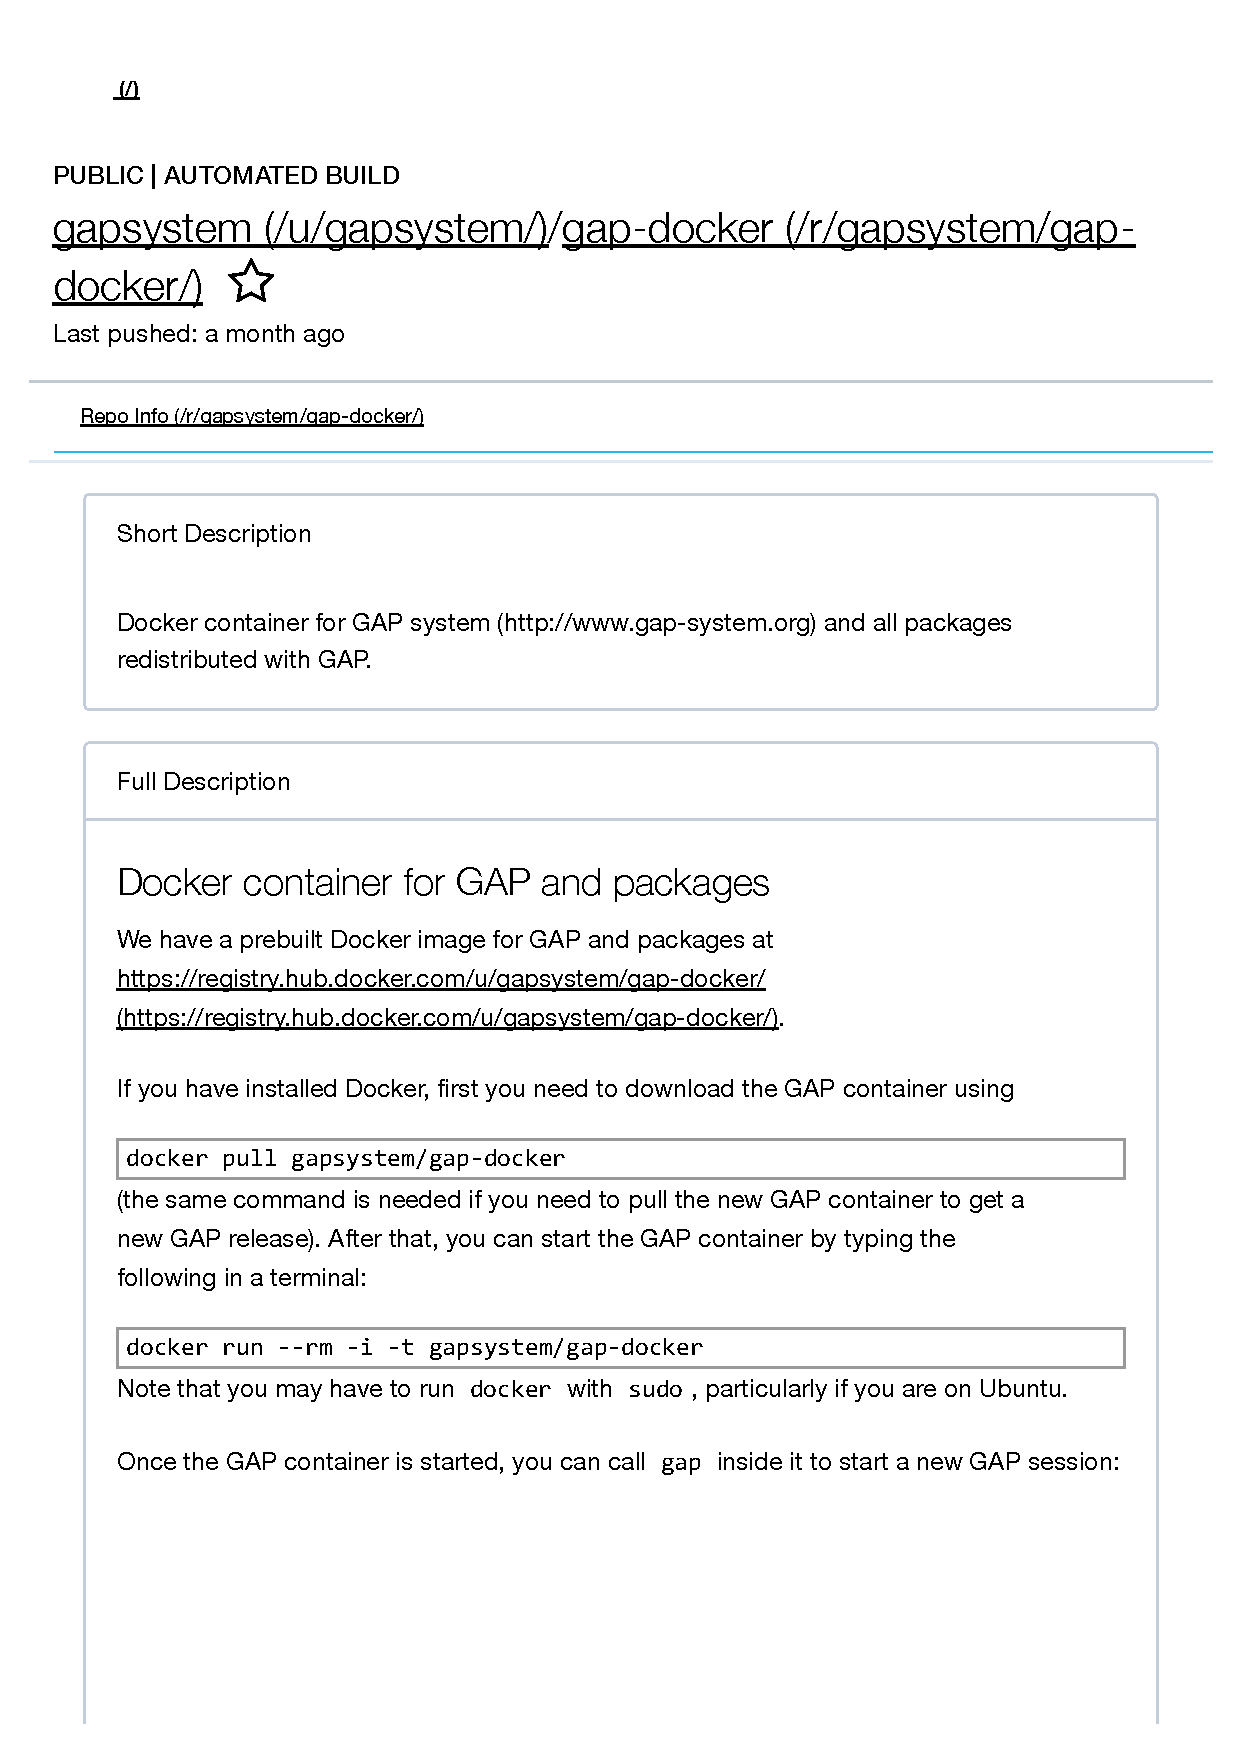
\includepdf[pages=-,scale=0.8,pagecommand={}]{examples/SCSCP-with-GAP-docker.pdf}
\section{Documentation on GAP SCSCP server for the number of isomorphism types of groups of order $n$}
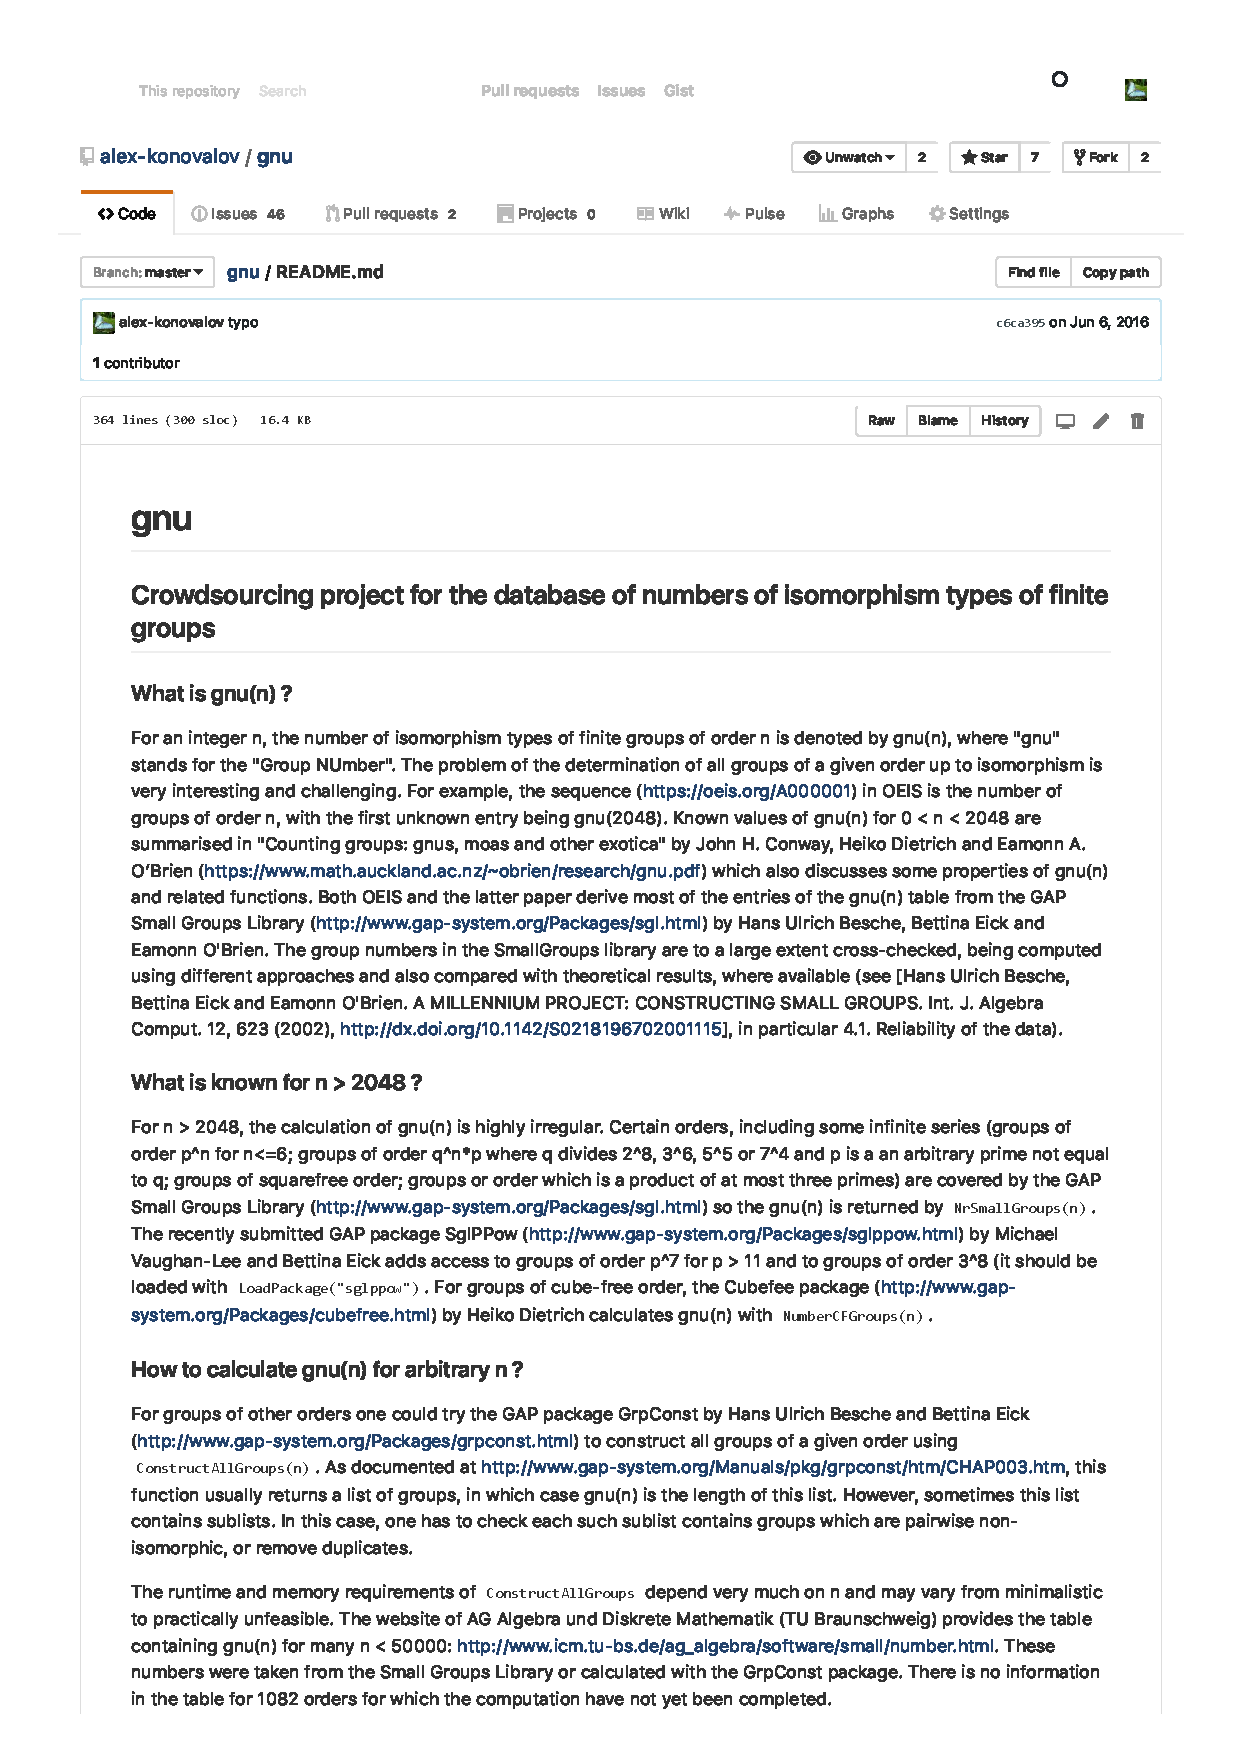
\includepdf[pages=-,scale=0.9,pagecommand={}]{examples/Gnu-SCSCP-server.pdf}
%TODO: Do we need to include manuals of GAP packages?
%\section{Documentation for GAP package OpenMath}
%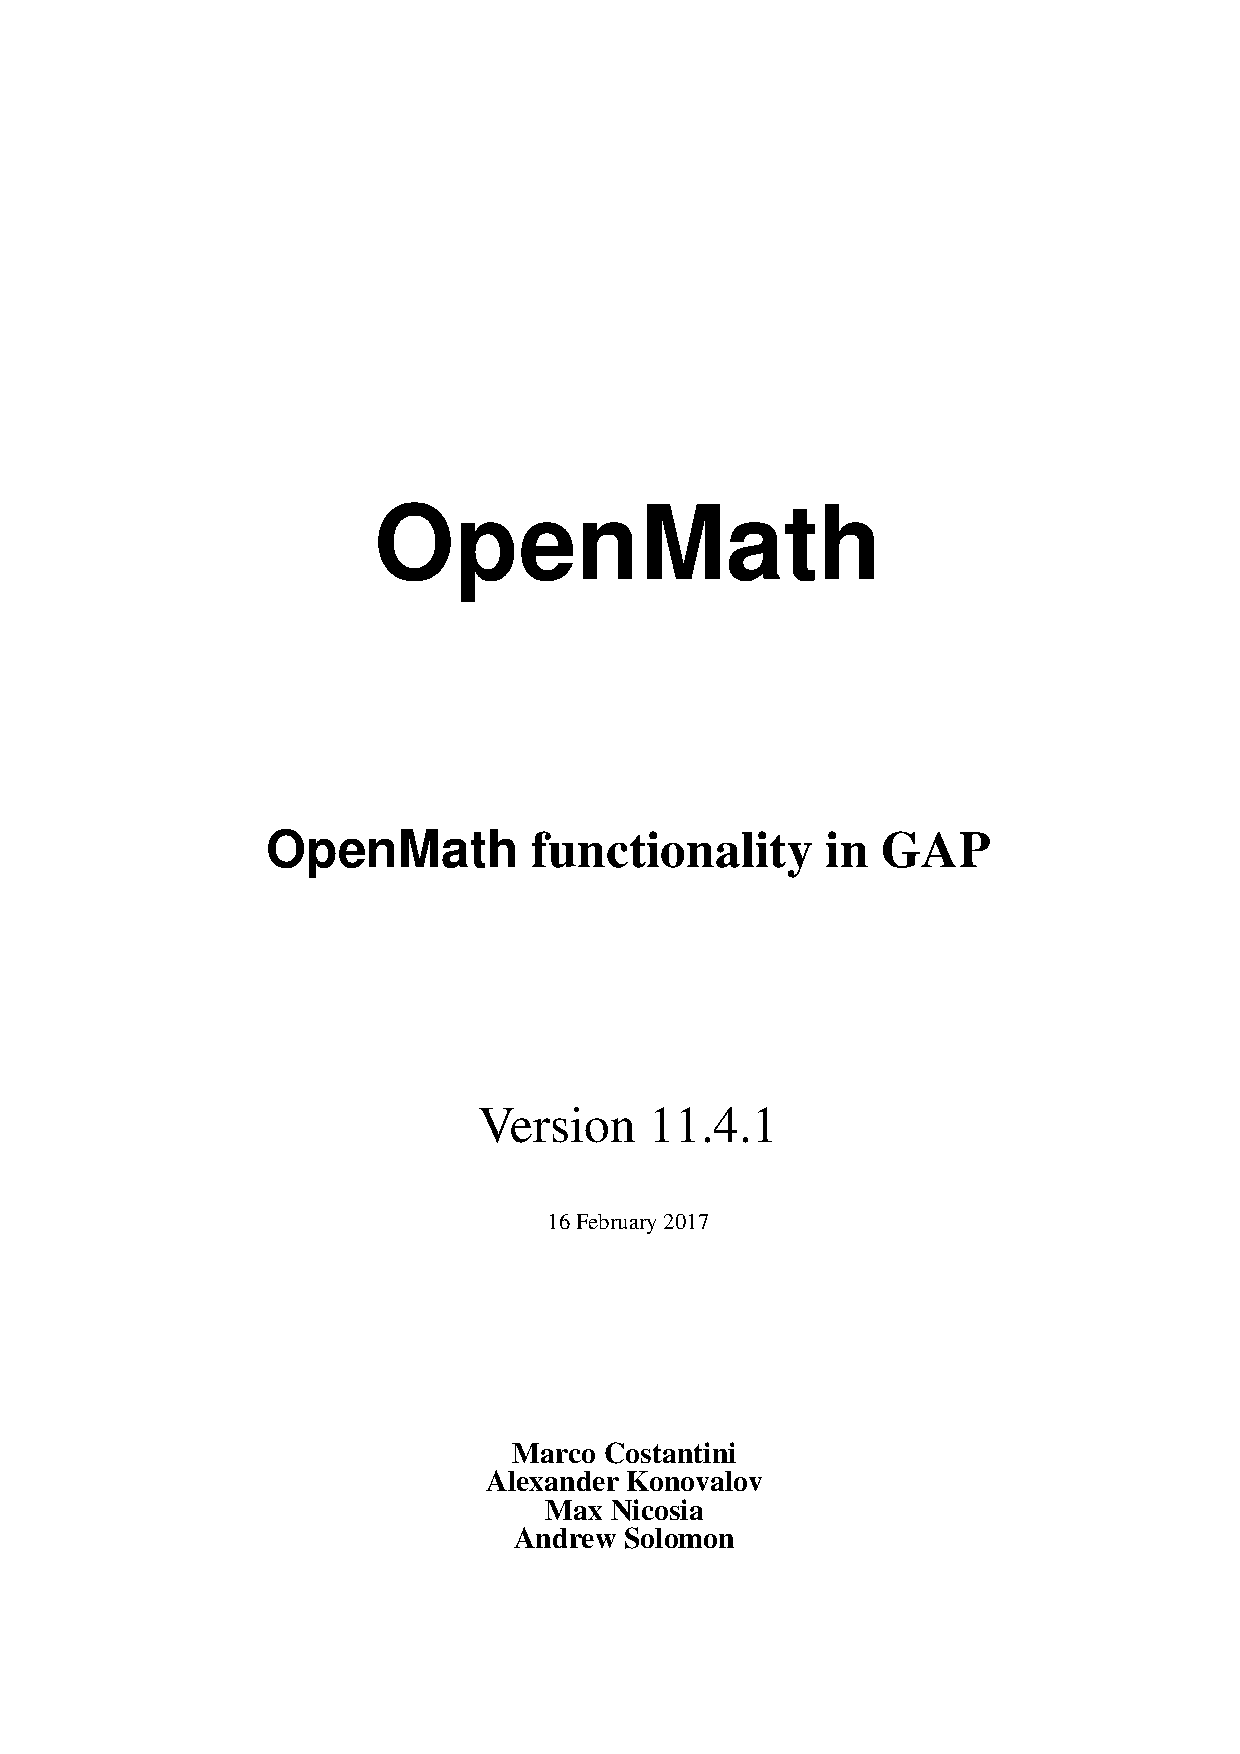
\includepdf[pages=-]{manuals/gap-openmath.pdf}
%\section{Documentation for GAP package SCSCP}
%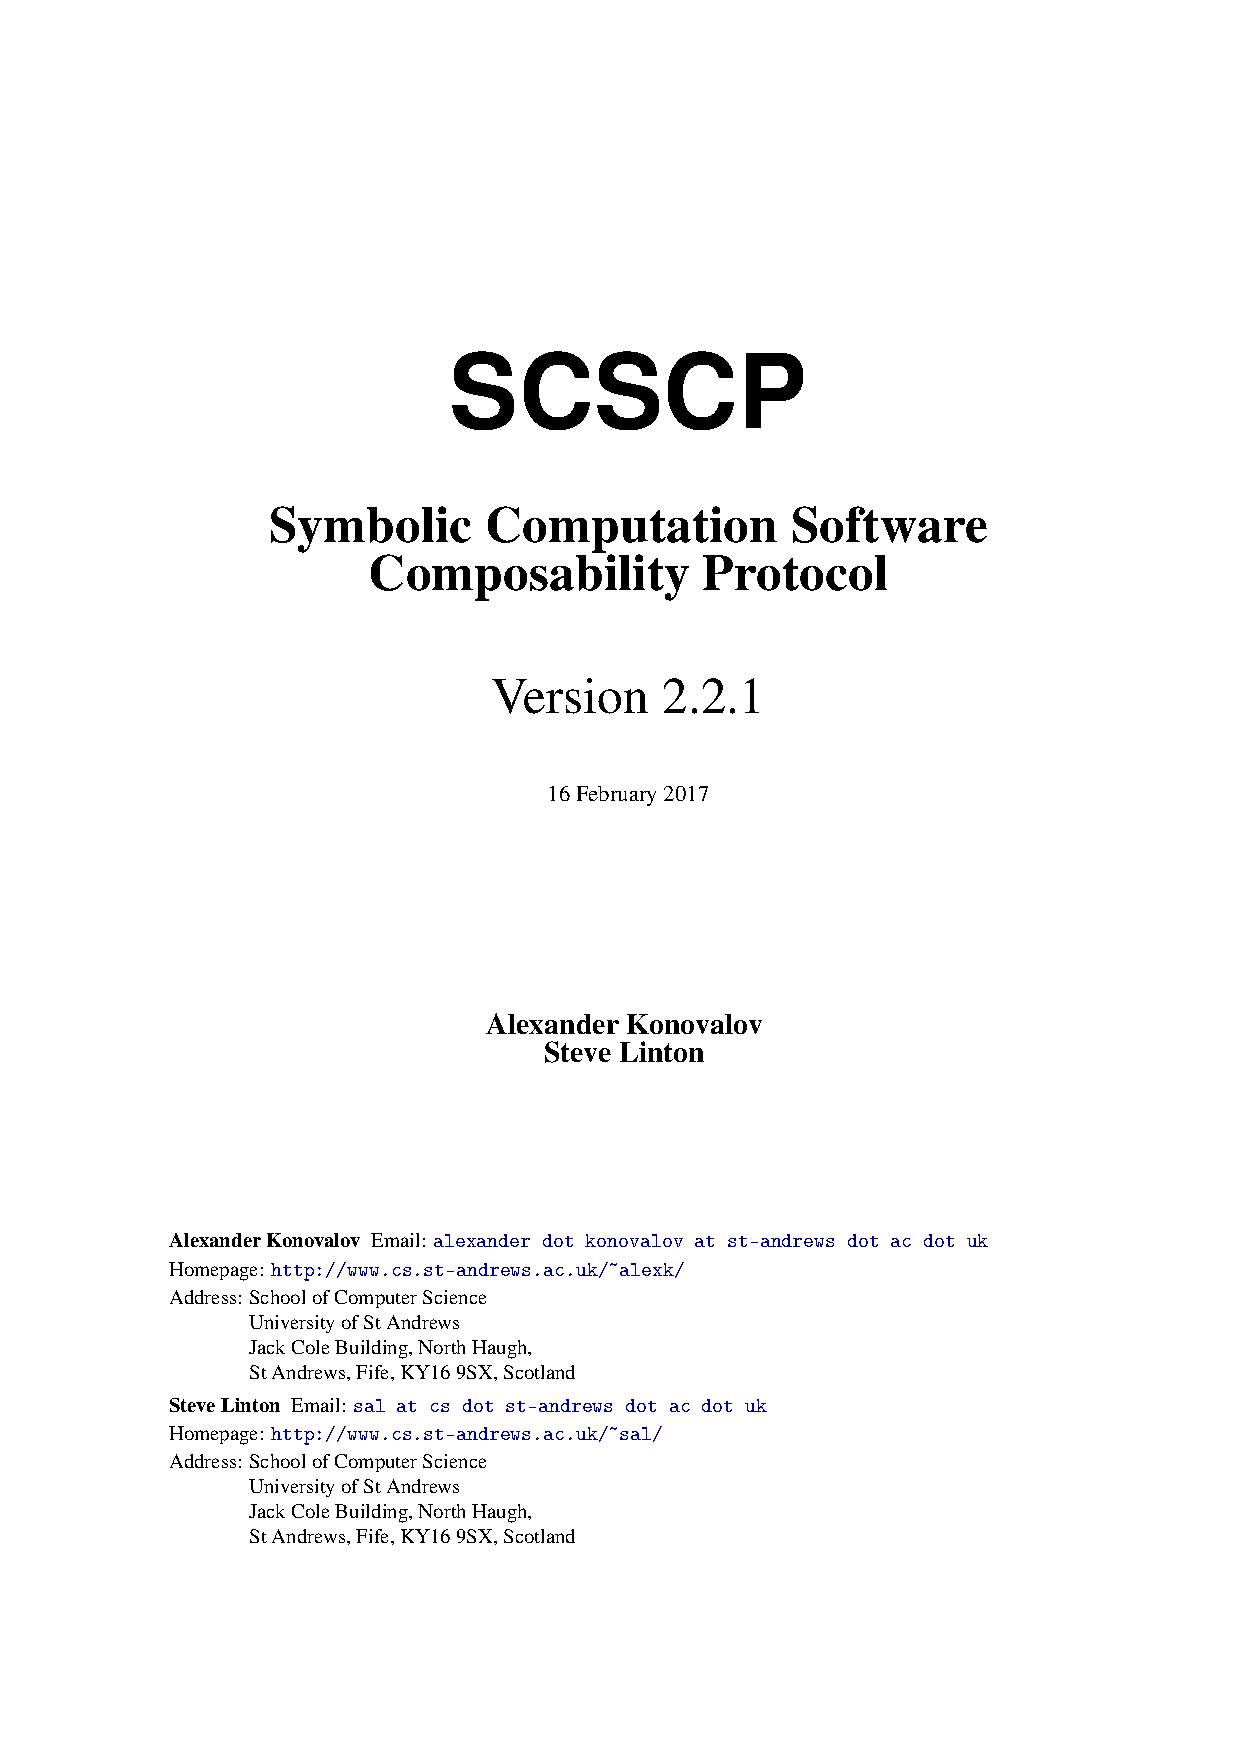
\includepdf[pages=-]{manuals/gap-scscp.pdf}

\end{document}

%%% Local Variables:
%%% mode: latex
%%% TeX-master: t
%%% End:

%  LocalWords:  githubissuedescription newpage tableofcontents newpage printbibliography
